\chapter{Analysis}
\label{chap:analysis}
% vysvetlit soucasny stav full textu v portalu
% kapitola by mela obsahovat pozadavky
%			co zmenit, co udelat a dodelat, co nedelat 
		% jake jsou pozadavky na vyhledavani, co ma byt vyhledavano
		% jak to ma byt vyhledavano
		% jak to nema byt vyhledavano
		% co by melo vyhledavani umet


This chapter focuses on the analysis of the state of the EEG/ERP Portal before making any changes to its full text search feature.

\section{Current State of Full Text Search}
\label{sec:currentStateFulltext}

%% Jaky je aktualni stav, jeho uvozeni
Currently, the EEG/ERP Portal application uses Hibernate Search as a mechanism to index chosen data stored in Oracle RDBMS.
% Jak je to v soucasne dobe zarizeno. Nedat to radsi do teorie?
Hibernate search provides the annotation interface which serves for indexing purposes. 
A subset of these annotations is used to mark indexed entities and fields withing them which should form the document in the index. Furthermore, a few field annotations enable to configure how the fields are later processed by specifying analyzers to be applied on those fields.

% pridat schema architektury?


By using Hibernate Search to implement full text search, the application is enforced to use Hibernate or JPA for data persistence \cite{Bernard:2008:HSA:1524089}.
Using any other technologies than these two results in a malfunctioning application.
The main drawback of using Hibernate Search in our case the inability to index data from different sources than the database. 
Since one of the requirements is to enable searching data from social networks, the current solution can hardly fulfill this requirement. 


% ???
%We do not have such control over indexed data (?) rozepsat

%% Jake jsou nevyhody soucasneho stavu
% index v pameti - jake jsou vyhody, nevyhody, rizika
In the current state of full text search, the indexed data are stored in memory. 
Keeping an in-memory index provides fast performance of searching because accessing data in memory is much faster than if data are stored on disk. 
A disadvantage of the in-memory index is that these data are lost every time the application server stops.
This is the reason why the index must be created each time the application starts running.
Furthermore, as the size of the index gets bigger, the available amount of memory may be insufficient.
The lack of memory then results in disk swapping which causes serious performance degradation.

Since Hibernate Search uses Lucene as a search library which is responsible for indexing and full text search, the created classes that represent full text search logic in the EEG/ERP Portal make a heavy use of the Lucene API.
Direct Lucene API usage is considered low-level for these purposes, the created code is more difficult to maintain and it is more likely that new bugs are introduced.
In the current state, for example, text highlighting of a subset of found results does not work as expected in some cases.

It is shown in Figure \ref{fig:architBeforeSolr} that the current implementation of full text search is, apart from its dependency on Hibernate, tightly coupled with the whole application. 


\begin{figure}[h]
	\centering
		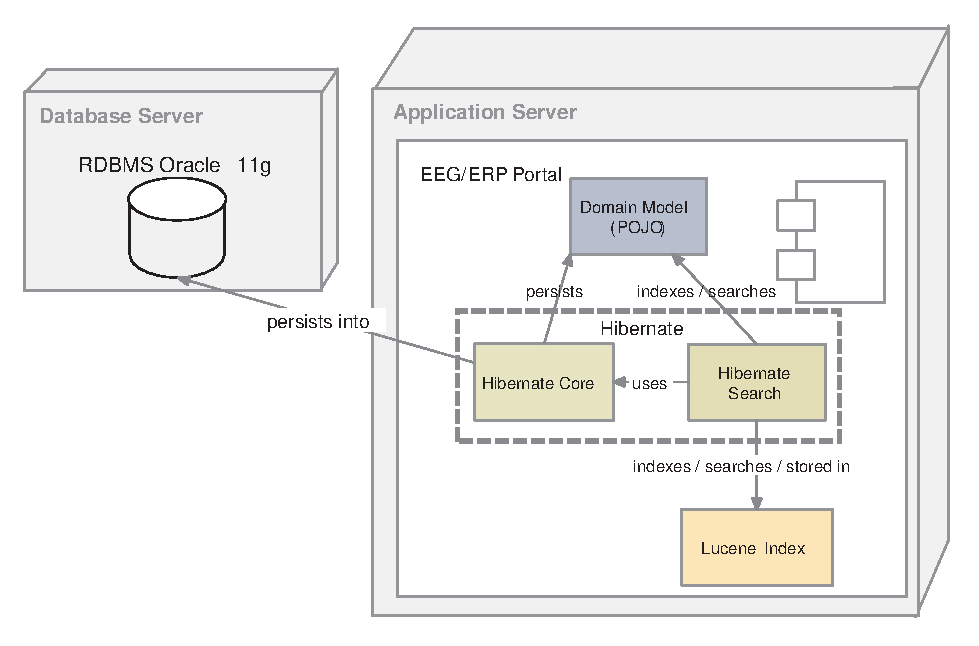
\includegraphics[width=1.00\textwidth]{figures/architBeforeSolr.eps}
	\caption{Architecture with Hibernate Search.}
	\label{fig:architBeforeSolr}
\end{figure}


%With the growing amount of indexed data, the full text search performance might go down as with limited amount of memory there is  not much space for scaling.




\section{Current State of Integration with Social Networks}

Currently, the EEG/ERP Portal is successfully integrated with its LinkedIn group. 
A user can use the EEG/ERP Portal to publish LinkedIn articles as well as to see all of them. 
Users can also log in to the EEG/ERP Portal via LinkedIn. 
Since LinkedIn uses the OAuth 2.0 security protocol for authentication, the OAuth authentication flow is implemented by using Spring Social.

%\section{Search Requirements}

%The current version of the EEG/ERP Portal uses Hibernate Search to implement the fulltext search feature. 
%This framework is sufficient for dealing with input data coming only from a database data source. 
%This is because of the fact that the technology is based on Hibernate, a powerful object-relational mapping framework. Hibernate %Search uses internally Lucene and Solr analyzers to provide the full text search itself.
%The full text search implementation suffers from several issues which are desired to be fixed.
%The highlighting functionality is required to be fixed because it does not work as expected in certain cases. 
%If phrases are searched, found phrases should be highlighted in the text as one piece.

\subsection{Desired Improvements of Full Text Search}


\subsubsection{Appearance}

The user interface of the page with search results should basically remain the same. 
As far as search forms are concerned, it is expected to have:

\begin{itemize}
	\item one search text field on the search page,
	\item another one in the header of each web page so the search can be executed from any page of the website.
\end{itemize}

\subsubsection{Search Functionality}

In terms of search features, there is a need to enable easier navigation among found results.
This is why faceting search based on result categories should be made.
Furthermore, synonym search is desired to allow finding also the results that contain defined synonymic keywords.
Moreover, wildcard search as well as using Boolean AND, OR and NOT operators for querying is required.

\subsection{Social Network Search}
% Duplicitni informace?
Since Hibernate Search is used as a technology responsible, among others, for data indexing, only the data stored in the relational database can be indexed. 
However, articles and other information found in the LinkedIn group of the EEG/ERP Portal have no direct connection to the database, so Hibernate Search cannot reach these data and therefore cannot save them to the index it keeps. 
A possible solution which partially solves this problem would be to keep duplicate records about the articles in the EEG/ERP Portal database. 
Apart from the problem with keeping three copies of basically the same information (the original article published on LinkedIn, its copy in the database and its representation in the Lucene index), those articles published directly from LinkedIn and not from the EEG/ERP Portal via a form would get unnoticed by the application and their corresponding documents in the index would not exist.


\section{Choice of Full Text Search Solution}

From the search engines listed in previous parts of the thesis and technologies on which the EEG/ERP Portal is based, the choice of the search engine can be restricted by the following criteria:

\begin{itemize}
	\item \textit{speed} - Based on the comparison made in chapter \ref{chap:engines}, the most performant search engines are ... and Lucene and all those search solutions built on Lucene. 
	However, speeds of the compared search engines, except for Xapian, differ only slightly. Due to their overall great performance, they can be considered a suitable solution with respect to this criterion.
	\item \textit{integration with the EEG/ERP Portal} - The EEG/ERP Portal is based on Java technologies and this is why search engines providing Java API are easier to be integrated to the working infrastructure and therefore preferred.
	\item \textit{other features and extensions} - Because full text search
engines as they are take care of indexing and searching data, it is desirable to have a set of built-in features, such as result highlighting, faceted search, synonym search or more-like-this search, to make building full text search easier.
 It is taken for granted by the end users to use the full text search with some of such features implemented. 
	\item \textit{independence on data sources} - The chosen search engine must be able to accept data from various sources and to not be limited to only one specific data source, such as relational database. T
	he reason behind this is the mentioned need to index LinkedIn articles as well as to enable further possible indexing scenarios in the future, such as indexing .pdf or XML files.
	\item \textit{independence on other technologies} - This criterion means that the search engine should not rely on a specific technology to be used. 
	Dependence of Hibernate Search on Hibernate or heavy orientation of Sphinx on MySQL may serve as the examples of the search engines which perform well if certain conditions are met, but cannot run or do not perform well if not. 
	\item \textit{community} - Numerous and active developer community also plays a big role in the final choice. 
	The bigger community around the search engine is, the higher is the chance that the engine development will not stop early, new features will be introduced and that found bugs will be resolved quickly. 
	Although relatively new one-man projects can look very promising and their future development is more likely to be managed by a still growing community, their stability is not guaranteed and hence their choice introduces a higher chance that
	A well documented project, many available tutorials and active user groups are a good sign of project stability and ensure that there will be probably someone willing to help to solve given problems.

\end{itemize}

The search engines were evaluated based on these criteria. This evaluations can be seen for reasons of clarity in table \ref{tab:ComparisonOfFullTextSearchEngines}

%TODO MODIFY the table.

\begin{table}[h!]
	\caption{Comparison of Full Text Search Engines.}
	\centering
	\scalebox{0.8} {
		\begin{tabular}{|c|c c c c c|}
		\hline

		\textbf{Search Engine } & \textbf{Speed} & \textbf{Integration} & \textbf{Extension} & \textbf{Independence} & \textbf{Community} \\
		\hline
		Indri & Excellent & \tick & \fail & \tick & 1 \\
		\hline
		Sphinx & Excellent & \tick & \fail & \tick & 3 \\
		\hline
		Lucene & Excellent & \tick & \tick & \tick & 5 \\
		\hline
		Zettair & Excellent & \fail & \fail & \tick & 1 \\
		\hline
		Xapian & Good & \tick & \tick & \tick & 1 \\ 

		\hline
		\end{tabular}
		}
	\label{tab:ComparisonOfFullTextSearchEngines}
\end{table}

% vysvetleni, co znamenaji jednotliva hodnoceni
It is worth mentioning that the last criterion, Community, cannot be evaluated in an exact manner. This criterion involves the size of mailing lists, the number of search results found on Google, number of related blog posts as well as the number of posts on specialized websites, such as \textit{Stack Overflow}.

The result of the comparison is to base the the EEG/ERP Portal full text search feature on the Lucene search library. As mentioned in Section \ref{sec:luceneBasedSolutions}, the Lucene-based search applications are in practice built by using more sophisticated search solutions (also mentioned in Section \ref{sec:luceneBasedSolutions}). 

\subsection{Chosing Lucene-based Solution}

From the solutions based on Lucene listed in section \ref{sec:luceneBasedSolutions}, it is obvious that Hibernate Search cannot be used due to the reasons that can be found in section \ref{sec:currentStateFulltext}.
Although both Solr and ElasticSearch are likely to be good full-text search solutions for the EEG/ERP Portal, it was decided to choose a more proved and mature alternative (by the time of making this decision, in November 2012). This is why ElasticSearch was favored to Solr.

\section{Using Solr} 

% http://blog.frankel.ch/solr-overview-from-a-beginners-point-of-view

% http://www.optimation.co.nz/optimation-blog/01-03-2011/open-source-faceted-searching-using-solr-and-solrj

% http://www.e-zest.net/blog/about-apache-solr/
	
% \subsection{How Solr Works}


\subsection{Installation}

The whole Solr distribution can be downloaded from the Solr website \cite{SolrHome}. 
It comes in a form of a .war archive. 
Apart from the Solr application itself, it also includes a set of configuration files.



\begin{figure}[h]
	\centering
		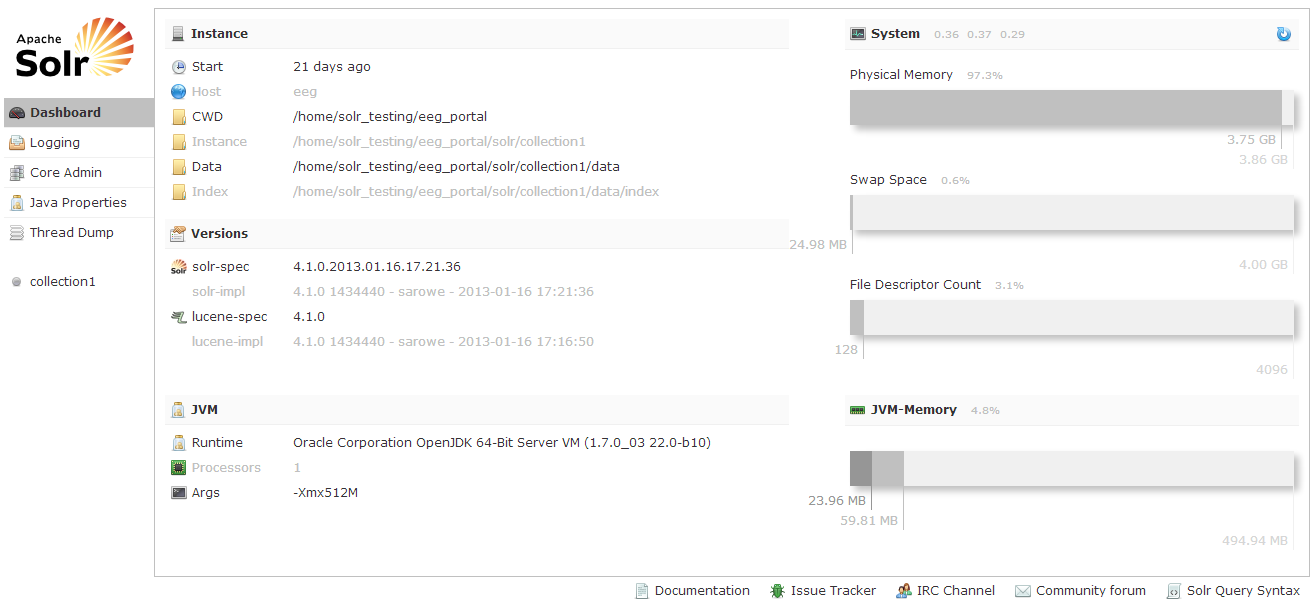
\includegraphics[width=1.00\textwidth]{figures/solrInterface.png}
	\caption{Solr User Interface.}
	\label{fig:solrInterface}
\end{figure}


%\section{Solr and NoSQL}


\subsection{Solr Index}

As told earlier, Solr follows the commonly used search engine terminology. 


\subsection{Solr Configuration}
% co se da nakonfigurovat


% snd HOTOVO
\subsection{General Ways of Integrating Solr}
%jake jsou hlanvi moznosti, uvest je.

There are basically two ways of how to integrate Solr with an existing application. The first way is based on configuration of periodically executed SQL queries that handle database indexing. To do this, the \textit{DataImportHandler} (DIH) tool is used. Another way is to apply a programmatic approach and to use a Java API called \textit{SolrJ}.



\subsubsection{DataImportHandler}
% opet co to je, na co se to pouziva, uvest jeho nevyhody

\textit{DataImportHandler} (DIH) offers fast indexing of data from a variety of sources, including relational databases. 
The extraction of database data for indexing is based on creating custom SQL queries.
The SQL queries serve as a mapping mechanism between query target attributes and document fields.

Although DIH configuration is straightforward to set and its indexing performance is excellent, it has several limitations and disadvantages:

\begin{itemize}

\item \textit{data model changes} - In order to index new data and to enable delta imports, i.e. to index only the changed data since last indexing, it is necessary to add a new time stamp column for each table whose data we wish to index. 
Each record of these new columns contains a time value of the last indexing activity.
Another issue that needs to be solved on the database level is managing deleted database records. There exist several methods to reflect the changes in the index and can be found for example in the Rafał Kuć's article \cite{Solr:DIHDelete}.

%\item \textit{need to manage deleted data} - After deletion of data in the database, certain actions must be taken to enable DIH to reflect these changes in the index. 
%One way to do this is to browse the documents in the index and compare their id values with id values of their matching database records. 
%If a document has no equivalent database record, it means that the record was deleted. 
%After the comparison, redundant documents in the index are identified. 
%This approach does not perform well.
%
%Another way is to add an extra column that captures deletion times. 
%Deletion times together with the record identification are added before the physical deletion of records. 
%DIH can then get all records from the last executed crawl. 
%An appropriate function and before delete trigger must be created for this solution. 

\item \textit{dealing with changes of the database schema} - If the database schema changes, all affected SQL queries must be rewritten in order to index the database correctly again. % SOLR schema changes are related to this point as well. 

\item \textit{code separation} - The logic in the form of the SQL queries is out of reach of the EEG/ERP Portal application logic since the queries must be written in a special configuration file managed by the Solr server.

\item \textit{for indexing only} - DIH is just an indexing tool that creates index documents. It cannot be used for retrieving the documents, so their searching must be implemented in a different way.

\end{itemize}



\subsubsection{SolrJ}
% co to je, co to umi, jake jsou jeho moznosti, proc by se melo pouzit

Solr provides a Java API for integration of Java applications with the Solr server called SolrJ API.
SolrJ client is a recommended way of how to integrate an existing Java application with the Solr server [zdroj]. % najit

SolrJ offers two possible ways of running Solr. Apart from the remote communication with the Solr server provided by the \texttt{HttpSolrServer} class, Solr can also be embedded within the EEG/ERP Portal application by running as the \texttt{EmbeddedSolrServer} instance. 
The latter option is generally not a recommended way to run Solr since Solr is in this case tightly bound to the resources of the running application. % najit info
Following the stated requirements, the embedded version of Solr is not a suitable option for the EEG/ERP Portal either.

\subsubsection{Maven Dependencies}

EEG/ERP Portal uses the Maven build automation tool. 
For both Solr and SolrJ, there are available Maven dependencies that can be added to the Maven \textit{pom.xml} file.
Listing \ref{listing:mavenSolrSolrJ} shows these added dependencies.

\begin{lstlisting}[language=XML, caption={Solr and SolrJ Maven Dependencies.}, label={listing:mavenSolrSolrJ}]
<dependency>
	<groupId>org.apache.solr</groupId>
  <artifactId>solr-core</artifactId>
  <version>4.1.0</version>
  <exclusions>
		<exclusion>
			<artifactId>slf4j-jdk14</artifactId>
      <groupId>org.slf4j</groupId>
    </exclusion>
  </exclusions>
</dependency>

<dependency>
	<groupId>org.apache.solr</groupId>
  <artifactId>solr-solrj</artifactId>
  <version>4.1.0</version>
</dependency>
\end{lstlisting}

% Uvest priklad instanciace solr serveru - beana

% \subsubsection{Running Solr}

% tyka se SolrJ
%HttpSolrServer and EmbeddedSolrServer


\section{Proposed System Architecture}

Based on the text from the preceding paragraphs, a new system architecture was proposed.
The architecture schema is depicted in Figure \ref{fig:solrNewArchitecture}.
Due to the needed interaction with the EEG/ERP Portal, SolrJ API is used as the most flexible alternative.
There are two Solr Server instances running.
One of them is used for maintaining indexed data of the production environment.
The second one is utilized for testing purposes.
Using a separate Solr test server was preferred to its application-embedded version due to the reasons described in previous text.


%% TODO uvest pro co se rozhodnout


\begin{figure}[h]
	\centering
		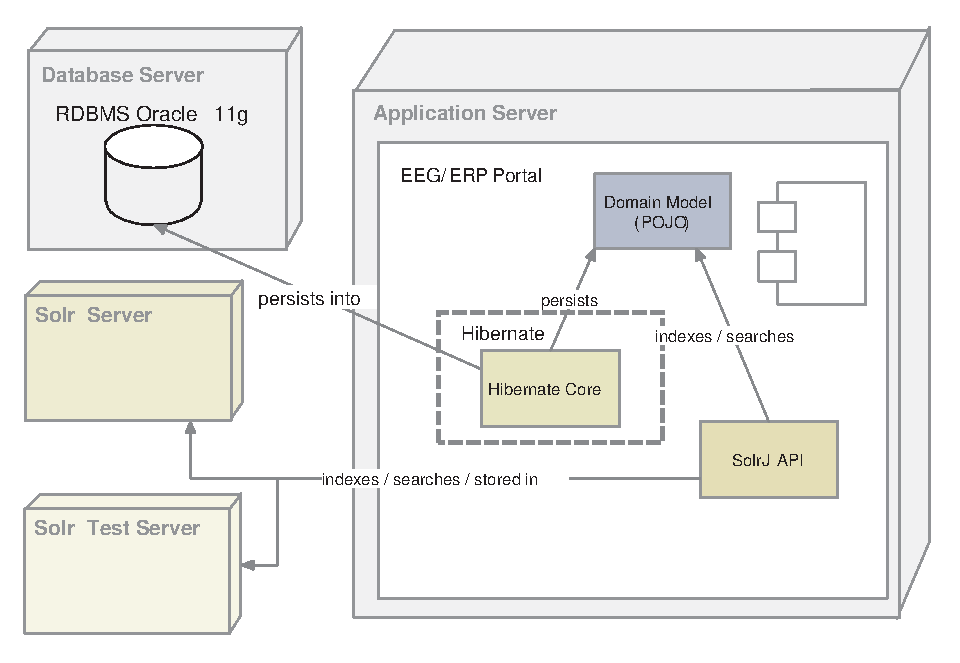
\includegraphics[width=1.00\textwidth]{figures/solrNewArchitecture.eps}
	\caption{Architecture with Solr Included.}
	\label{fig:solrNewArchitecture}
\end{figure}
